%!TEX root = ../thesis.tex
%*******************************************************************************
%****************************** Third Chapter **********************************
%*******************************************************************************
\chapter{Filogenética, propiedades fisicoquímicas y minería de datos aplicados al diseño de mutaciones en secuencias de proteínas \label{cap4}}

% **************************** Define Graphics Path **************************
\ifpdf
    \graphicspath{{Chapter4/Figs/Raster/}{Chapter4/Figs/PDF/}{Chapter4/Figs/}}
\else
    \graphicspath{{Chapter4/Figs/Vector/}{Chapter4/Figs/}}
\fi

Uno de los problemas de mayor relevancia para el campo de la ingeniería de proteínas, es el diseño inteligente de mutaciones, con el fin de obtener una propiedad fisicoquímica, mejorar las características o adicionar una nueva funcionalidad. Sin el hecho de incurrir en grandes costos económicos, de recursos humanos y computacionales.

En la sección \ref{cap1:sec1}, se mencionó que existen dos puntos de vista a la hora del diseño de mutaciones: Evolución dirigida y el diseño racional de proteínas. Sin embargo, ambas presentan el problema del poco espacio de exploración que pueden abarcar. A partir de ello, y con el fin de disminuir los tiempos experimentales y aumentar el espacio de búsqueda, métodos computacionales fueron implementados como herramientas de apoyo al diseño de mutantes. 

A pesar de la existencia de dichos métodos, para aquellos basados en potenciales de energía y en simulaciones Monte Carlo, el tiempo computacional necesario para explorar la totalidad de mutaciones en una proteína en particular, escala a nivel cuadrático, siendo elevado y de limitado acceso para usuarios en general.

Una alternativa a los métodos computacionales basados en estrategias de potenciales de energía, son aquellos que emplean técnicas de minerías de datos y algoritmos de aprendizaje. Sin embargo, estos, principalmente se enfocan en el estudio de la estabilidad de la proteína ante sustituciones de aminoácidos. Por otro lado, los principales enfoques en cuanto a caracterización de residuos, se centran en propiedades termodinámicas y el ambiente, no siendo considerados conceptos filogenéticos ni propensión a cambios. 

Tal como se expuso en el capítulo \ref{cap3}, la codificación de secuencias lineales puede ser realizada a través del uso de propiedades fisicoquímicas y posterior digitalización de éstas, aplicando transformadas de Fourier, esto último, permite caracterizar el ambiente y el aporte hacia las características que brindan los residuos, debido a las propiedades del espacio de frecuencias y el espectro como tal. 

Apoyados en dicha codificación y centrados en la utilización de algoritmos de aprendizaje supervisado para el entrenamiento de modelos de clasificación o regresión, y utilizando la metodología expuesta a lo largo del capítulo \ref{cap2}, además del uso de herramientas computacionales como filtros de diseño. Se propone durante este capítulo el diseño e implementación de una herramienta computacional, basada en técnicas de minería de datos y aprendizaje de máquinas, que permita el diseño de mutaciones en variantes con características deseadas.

\section{Hipótesis}

En base al planteamiento del problema y a la motivación existente por el desarrollo de una herramienta computacional para el diseño de mutaciones, se plantea la siguiente hipótesis.\\

\textit{La digitalización de las propiedades fisicoquímicas por medio de transformadas de Fourier, en conjunto con algoritmos de aprendizaje supervisado, en combinación con herramientas computacionales para evaluar estabilidad y propensión, serán un enfoque suficiente para el desarrollo de una herramienta de diseño de mutaciones}

\section{Objetivos}

Dada la hipótesis planteada y en vista del desafío considerado, se exponen a continuación el objetivo general y los objetivos específicos.

\subsection{Objetivo general}

Diseñar, implementar, testear y depurar herramienta computacional para el diseño de mutaciones puntuales en variantes de proteínas, enfocada en el uso de minería de datos y
aprendizaje supervisado y en la generación de estrategias de filtro de mutantes con respecto a
caracteristicas termodinámicas y filogenéticas.

\subsection{Objetivos específicos}

Del objetivo general, nacen los siguientes objetivos específicos.

\begin{enumerate}
	
	\item Implementar, evaluar y analizar, sistema de codificación de secuencias lineales por medio de propiedades fisicoquímicas y el uso de digitalización a partir de transformadas de Fourier.
	\item Entrenar, evaluar y validar modelos basados en algoritmos de aprendizaje supervisado, con descriptores enfocados en espectros de frecuencias de propiedades fisicoquímicas.
	\item Diseñar e implementar módulo de filtro de mutaciones por medio de propensión de la mutación y efecto en la estabilidad que provoque la sustitución.
	\item Implementar y evaluar flujo de trabajo para nuevas mutaciones, mostrando el desempeño del modelo y los valores asociados a ésta, junto con otras características de	interés.
	
\end{enumerate}

\section{Métodología propuesta}

Dada la hipótesis planteada y los objetivos propuestos, se diseña una metodología que contemple tanto la generación de la herramienta computacional, como el desarrollo de los modelos y su entrenamiento.

Un esquema representativo de los componentes principales de la metodología y cómo estos interactúan se expone en la Figura \ref{cap4:fig1}. El proceso general, se puede dividir en dos etapas: Generación de los modelos y Evaluación de nuevas mutaciones. En la primera etapa, se contempla un conjunto de datos, el cual es sometido a la etapa de digitalización, posterior a ello, se entrenan los modelos considerando como descriptores los espectros de frecuencia, para luego evaluar su desempeño. En la segunda etapa, nuevas mutaciones son propuestas y evaluadas en una etapa de filtro, aplicando criterios de estabilidad y propensión filogenética, para luego, someterse a los modelos predictivos generados y así evaluar si la mutación tendrá el efecto deseado o no.


\begin{figure}[!h]
	
	\centering
	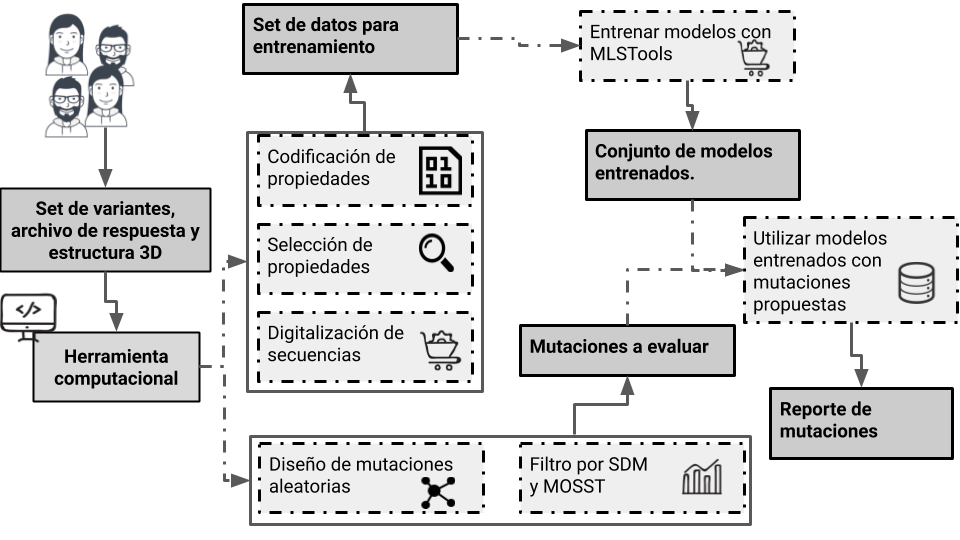
\includegraphics[scale=.4]{fig1.png}
	\caption{Esquema representativo de la metodología propuesta para el diseño de mutaciones aplicando herramienta computacional a desarrollar}
	\label{cap4:fig1}
\end{figure}

Un punto importante a evaluar, consiste en el hecho que el conjunto inicial de datos debe ser lo suficientemente representativo en cuanto a la diversidad de ejemplos, es decir, si se evalúa la presencia o ausencia de una característica, no debe existir un desbalance entre ellas, ya que provocaría un sobreajuste en el modelo, tendiendo a predecir sobre la característica de mayor proporción.

A continuación, se describe el conjunto de datos inicial, seguido de las etapas que componen la metodología y finalizando con la estrategia para el diseño e implementación de la herramienta computacional.

\subsection{Conjunto de datos}

El conjunto de datos corresponde a un grupo de variantes de una misma proteína, ordenados en un archivo en formato *.fasta\footnote{Formato de texto plano para la representación de secuencias.}, siendo la primera secuencia la proteína original, y el resto de secuencias las variantes con mutaciones reportadas. Además del conjunto de secuencias, es necesario un archivo en formato *.csv con la variable respuesta asociada a la variante, es decir, el valor de la propiedad fisicoquímica, característica, funcionalidad, etc., que provoca la mutación. Esto con el fin, de poder asignárselo a la secuencia y entrenar los correspondientes modelos. 

Adicional a ambos inputs, se requiere de un archivo *.pdb el cual contenga la estructura de la proteína original, o en su defecto, el código PDB de la misma, esto debido a que la etapa de filtro, utiliza SDM como método de análisis de estabilidad de la proteína ante sustituciones de residuos, siendo un input para ésta, la estructura 3D.

\subsection{Digitalización de secuencias lineales}

A partir del conjunto de secuencias, los residuos son codificados aplicando las propiedades fisicoquímicas descritas en la base de datos AAindex \cite{Kawashima2000}, considerando la totalidad de propiedades descritas. Para ello, se implementarán scripts bajo el lenguaje de programación Python, los cuales tomen los residuos de cada secuencia y los transformen a un vector de tamaño $n$ el cual corresponde a la cantidad de propiedades descritas en la base de datos. De esta manera, por cada secuencia se crea una matriz de tamaño $r \times n$ donde $r$ representa la cantidad de residuos en la secuencia.

Dada esta matriz $r \times n$, se aplican técnicas de reducción de dimensionalidad y análisis de características, con el fin de seleccionar las propiedades fisicoquímicas más informativas y que generarían un aporte al entrenamiento de modelos. Debido a que son $s$ secuencias existentes en el set de datos, se tendrán $m$ propiedades fisicoquímicas por cada secuencia en el conjunto de elementos. La selección se basará en las propiedades consenso que abarquen la totalidad de las secuencias. 

Es importante mencionar, que se espera que las propiedades informativas se mantengan a lo largo de la secuencia original y las variantes, ya que, cambios puntuales en los residuos, no alterarán de manera significativa la varianza que generen al conjunto de datos, alterando el orden de prioridad de las propiedades asociadas.

Una vez seleccionadas las propiedades fisicoquímicas a utilizar, se digitalizará su valor, con el fin de formar espectros de frecuencia asociados a dicho elemento; así, debido a que la selección previa, permite determinar un número $p$ de propiedades informativas, por cada secuencia $s$ en el conjunto de datos, se tendrán $p$ espectros de frecuencias. Estos espectros se obtienen a partir del uso de Transformadas rápidas de Fourier (FFT por sus siglas en inglés) \cite{brigham1988fast}, para lograr dicha conversión, se implementarán scripts bajo lenguaje de programación Matlab, los cuales, reciban como entrada el conjunto de propiedades por cada secuencia y retornen los espectros de frecuencia por cada propiedad. 

Finalmente, scripts basados en lenguaje de programación Python, completarán el conjunto de datos, considerando los espectros de frecuencia, seguidos de la respuesta que estos conllevan. De esta forma, generando el set de datos para el entrenamiento de modelos.

\subsection{Entrenamiento de modelos}

Los modelos se basarán en algoritmos de aprendizaje supervisado y se utilizará la misma metodología de exploración y selección de modelos basados en sus medidas de desempeño, expuestos en el capítulo \ref{cap2}. Se destaca que, el tipo de algoritmo a utilizar, depende de las características de la respuesta que se esté evaluando, es decir, si la respuesta presenta una distribución continua, se utilizarán los métodos basados en regresión, en caso contrario, se utilizarán algoritmos basados en clasificación.

Con respecto al desbalance de clases, éste se evaluará de la misma forma expuesto en el capítulo \ref{cap2}, además, las respuestas del tipo continua serán analizadas mediante la evaluación de outliers y la tendencia a distribución normal que presente.

El desempeño de los modelos, será obtenido a partir de lo expuesto en el capítulo \ref{cap2}. Uno de los puntos importantes a considerar es el valor de estas medidas. Modelos de clasificación con medidas inferiores serán descartados y requerirán un nivel de análisis más detallado. Por otro lado, modelos de regresión con coeficientes de correlación inferiores a 0.6, también implica que deben ser analizados de la misma forma. De esta forma, se asegura un cierto nivel de confianza a la hora de aplicar los modelos. No obstante, dado a que a la metodología planteada en el capítulo \ref{cap2} mejora las medidas de desempeño de los modelos iniciales, se espera que los casos expuestos de descarte no ocurran.

\subsection{Diseño de mutaciones}

Una vez los modelos se encuentren entrenados, será posible utilizarlos para evaluar nuevas mutaciones. Para ello, y con el fin de testear la herramienta, se implementará un script que permita mutar todas las posibilidades en cada residuo de la secuencia, es decir, para el residuo $i$ se sustituirá 19 veces, en caso de que la mutación ya se encuentre reportada, ésta será descartada. 

Una vez se tenga este conjunto de mutaciones, se aplicará un filtro basado en la propensión filogenética de dicha mutación y cómo afecta a la estabilidad el cambio propuesto. Para ello, se implementará servicios API (Application Programming Interface) que consuman las herramientas SDM \cite{Pandurangan2017} y MOSST \cite{Olivera-Nappa2011}, los cuales permitirán mencionar si la mutación es viable filogenéticamente y no provoca cambios en la estabilidad. Esto, generará una reducción de elementos en el conjunto de datos a estudiar, debido a que, no todas las mutaciones serán factibles. 

Ya con las mutaciones factibles, se codificará las secuencias de las variantes utilizando el método descrito previamente y aplicando las propiedades fisicoquímicas seleccionadas, con el fin de obtener los espectros correspondientes. 

Una vez obtenidos los espectros, se someten a los modelos entrenados y se obtiene la respuesta de interés, en base a las características del modelo. Se destaca que las respuestas serán reportadas en torno a intervalos de confianza, para métodos continuos, y, en forma de probabilidades, para el caso de respuestas categóricas.
 
\subsection{Implementación herramienta computacional}

La herramienta computacional será diseñada siguiendo el patrón de diseño Modelo-Vista-Controlador (MVC) \cite{krasner1988description} e implementada utilizando el paradigma de Programación Orientada a Objetos (POO) \cite{wegner1990concepts}, además, debido a que el componente de la vista, será asociado a interfaz web, se utilizará la arquitectura Cliente-Servidor, con el fin de responder las solicitudes y ejecutar las acciones correspondientes. El uso de POO es debido a que permite una mayor estandarización de los módulos y facilita su re usabilidad, además de la comprensión y simpleza a la hora de programar dado a su cercanía con la realidad y al poder de abstracción que posee.

Con respecto al patrón de diseño, se  expone  a continuación, cuáles serán los principales elementos en cada componente, además de sus características y qué comprenden cada uno de estos.

\subsubsection{Modelo}

El modelo corresponde al conjunto de scripts y módulos que contienen toda la lógica de la herramienta y las funcionalidades principales, se hace alusión a que forma parte del "back-end" de la aplicación. 

En este caso, se compondrá de los módulos de codificación, procesamiento de datos, entrenamiento de modelos, diseño de mutaciones y uso de servicios para la ejecución de MOSST y SDM, así como también los módulos de gestor de usuarios, notificaciones vía email, etc. Será implementado bajo el lenguaje de programación Python y utilizará algunas rutinas desarrolladas en Matlab. A su vez, cada módulo y sus componentes serán diseñados bajo el paradigma de Programación Orientada a Objetos y se utilizarán librerías externas como Pandas \cite{mckinney2010data} para la manipulación del conjunto de datos, Numpy \cite{van2011numpy} y Scipy \cite{oliphant2007python} para los análisis estadísticos y Scikit-Learn \cite{pedregosa2011scikit} para el entrenamiento de modelos.

\subsubsection{Controlador}

El controlador, hace referencia al gestor de las solicitudes de usuario desde la vista y recibe las respuestas de dichas solicitudes por parte del modelo, con el fin de ser expuestas al usuario. 

Para este caso, el controlador se dividirá en dos componentes principales: Controlador de acciones en la vista y Controlador de respuestas en el modelo. El primero, será implementado en JavaScript y tendrá funcionalidades asociadas a jQuery, mientras que el segundo, será desarrollado bajo el lenguaje de programación Php. 

La gran diferencia entre ambos, radica en el hecho de dónde se ejecutan, el primero, se encuentra principalmente condicionado por las acciones del usuario y su ejecución es en el navegador. Mientras que el segundo es una consecuencia del primero, es decir, una vez que se reciben las solicitudes, se establece la comunicación hacia el servidor por medio de Ajax (Asynchronous JavaScript And XML) y esto permite la ejecución del segundo, el cual, entrega una respuesta en formato JSON (JavaScript Object Notation), la que es capturada por el primero, y mostrada al usuario.

\subsubsection{Vista}

La vista, es el componente de visualización de la herramienta, es decir, es el componente en el cual el usuario puede interactuar, levantar solicitudes y exponer los resultados o respuestas que entregue el controlador y es conocido como "front-end".

Con el fin de poder representar las secciones principales que tendrá la herramienta, a continuación se exponen un conjunto de mockups (maqueta de diseño), en los cuales se exponen cuáles serán las principales funcionalidades y cómo se verán los resultados.

\subparagraph{Generador de jobs\\\\}

Los jobs, son los eventos generados asociados a un usuario y la carga de un conjunto de datos, los cuales deben ser codificados y entrenados los modelos, con el fin de evaluar las mutaciones posibles. Un esquema representativo del formulario asociado a la generación de jobs se aprecia en la Figura \ref{cap4:fig2}.

\begin{figure}[!h]
	
	\centering
	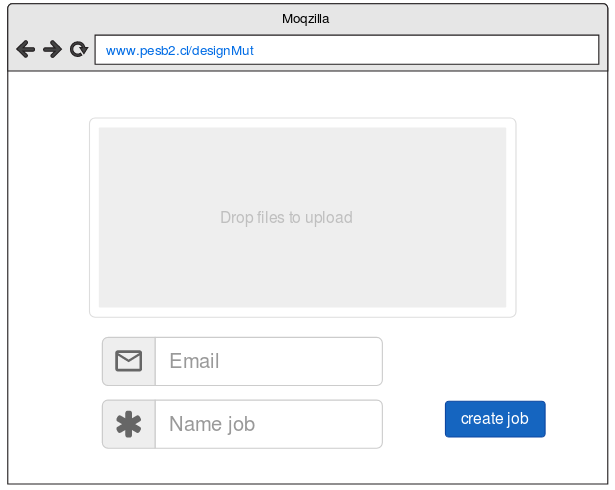
\includegraphics[scale=.4]{fig2.png}
	\caption{Esquema representativo interfaz de creación de jobs.}
	\label{cap4:fig2}
\end{figure}

En una primera instancia, el usuario deberá subir los archivos necesarios para entrenar los modelos, estos corresponden al conjunto de secuencias, el archivo de respuestas y la estructura 3D en formato *.pdb. Una vez suba los archivos, deberá ingresar el correo electrónico y el nombre del trabajo, esto para que él pueda identificarlo en el sistema. Cuando el usuario pulse el botón "create job", el sistema procesa la data y genera un ID asociado al identificador único del Job, posterior a ello, lo agrega al sistema de colas en el cual será procesado una vez le corresponda. Visualmente, el sistema retorna dicho ID, mostrándose en la interfaz y se notifica vía correo electrónico el estado del job, así como las notificaciones correspondientes del mismo.

\subparagraph{Buscador de jobs\\\\}

Adicional a la sección de crear jobs, la herramienta computacional permite buscar los trabajos generados, estos pueden encontrarse en 4 estados:

\begin{itemize}
	
	\item \textbf{Creado}: se refiere al estado en el que el usuario sube la data y se ancla al sistema de colas.
	\item \textbf{En ejecución}: el job está siendo ejecutado por la herramienta computacional. 
	\item \textbf{Finalizado}: el job fue ejecutado y es posible ver los resultados obtenidos.
	\item \textbf{Cancelado}: el job fue cancelado por el usuario.
\end{itemize}

Los jobs, pueden ser buscados en la interfaz del buscador de la herramienta web, mediante el ID o el nombre, ambos, son notificados vía correo electrónico, ya sea ante cambios de estado que éste sufra, o, al momento de crearse. Finalmente, una representación general del buscador, se observa en la Figura \ref{cap4:fig3}.

\begin{figure}[!h]
	
	\centering
	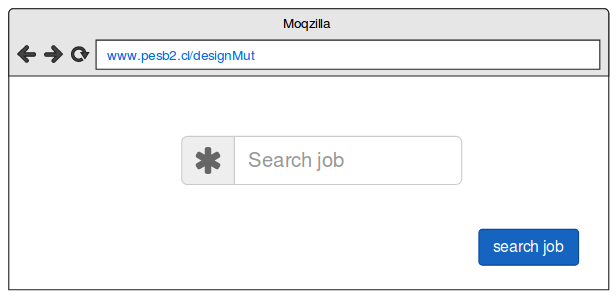
\includegraphics[scale=.4]{fig3.png}
	\caption{Esquema representativo interfaz de búsqueda de jobs.}
	\label{cap4:fig3}
\end{figure}

\subparagraph{Visualizador de resultados\\\\}

Una de las visualizaciones más relevantes, corresponde a los resultados involucrados en todo el proceso, estos, abarcan las propiedades fisicoquímicas estudiadas, los espectros de frecuencia y los residuos relevantes, los entrenamientos de los modelos y el listado de mutaciones favorables a evaluar. Un resumen general de los resultados esperados y la muestra de estos, es listada a continuación.

\begin{itemize}
	
	\item \textbf{Descripción general}: Se genera una visualización del conjunto de secuencias y la distribución o frecuencia de la variable respuesta, se expone un resumen del conjunto de datos y se muestran patrones relacionados a alineamientos múltiples de secuencia. Además de una visualización de la proteína de interés, en su estructura 3D y las sustituciones que exhiben cada variante. Esto puede observarse en la Figura \ref{cap4:fig4}.
	
	\begin{figure}[!h]
		
		\centering
		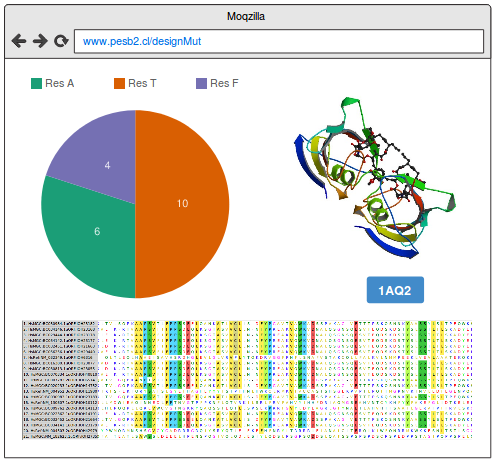
\includegraphics[scale=.5]{fig4.png}
		\caption{Esquema representativo interfaz de descripción general del conjunto de datos.}
		\label{cap4:fig4}
	\end{figure}
	
	
	\item \textbf{Propiedades fisicoquímicas}: Una representación de las propiedades fisicoquímicas abarca cuáles fueron las seleccionadas y las definiciones de éstas, por otro lado se expone el aporte a la varianza que éstas presentan y cómo varían por cada secuencia. Un esquema representativo de diseño de la interfaz, puede observarse en la Figura \ref{cap4:fig5}.
	
	\begin{figure}[!h]
		
		\centering
		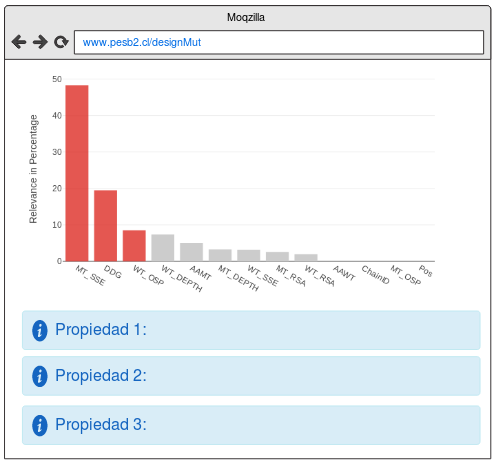
\includegraphics[scale=.5]{fig5.png}
		\caption{Esquema representativo interfaz de visualización de propiedades fisicoquímicas.}
		\label{cap4:fig5}
	\end{figure}
	
	\item \textbf{Espectros de frecuencia}: Se exponen el conjunto de digitalizaciones de las propiedades fisicoquímicas, asociados a los residuos que brindan la mayor caracterización y cómo estos inciden en el espectro. En la Figura \ref{cap4:fig6}, se expone un esquema de la visualización de los espectros, junto a los residuos relevantes.
	
	\begin{figure}[!h]
		
		\centering
		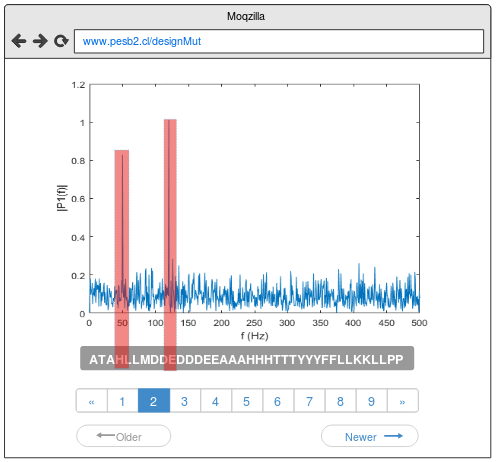
\includegraphics[scale=.5]{fig6.png}
		\caption{Esquema representativo interfaz de visualización de espectros de frecuencias y residuos relevantes.}
		\label{cap4:fig6}
	\end{figure}
	
	\item \textbf{Entrenamiento de Modelos}: Los modelos se exponen asociados a las medidas de desempeño obtenidas y los miembros participantes en el conjunto de modelos. Esto es debido a que se utilizará la estrategia expuesta en el capítulo \ref{cap2}, por lo que se obtiene un sistema de meta-modelos, cuyo esquema representativo de visualización se observa en la Figura \ref{cap4:fig7}. 
	
	\begin{figure}[!h]
		
		\centering
		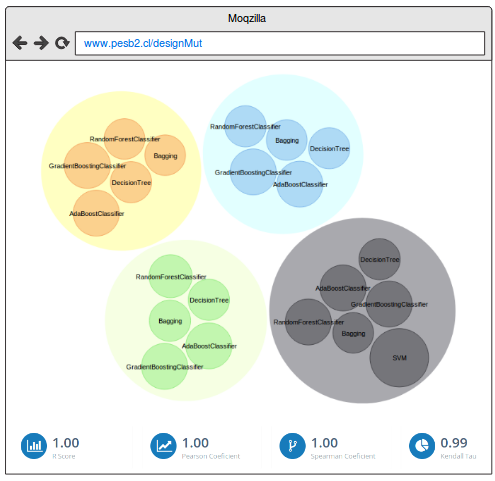
\includegraphics[scale=.5]{fig7.png}
		\caption{Esquema representativo interfaz de visualización de los meta modelos y sus medidas de desempeño.}
		\label{cap4:fig7}
	\end{figure}
	
	\item \textbf{Mutaciones propuestas}: Para el conjunto de datos, se proponen diferentes mutaciones, evaluadas con respecto a la respuesta y factibilidad de éstas, a su vez, se exponen estadísticas asociadas a qué residuos son más factibles de mutar en base a las posiciones de estos.
	
\end{itemize}


\subsection{Consideraciones generales}

Como consideraciones generales, se tiene que el conjunto de secuencias o variantes a estudiar, debe poseer una respuesta reportada, es decir, la variable de interés debe conocerse de ante mano, con el fin de poder entrenar los modelos de clasificación o regresión y así poder analizar nuevas mutaciones. 

Por otro lado, la secuencia original, debe presentar su estructura en formato *.pdb, ya que, se requiere para el uso de SDM, la cual es la herramienta de filtro asociada a la estabilidad de la proteína con respecto a los cambios o sustituciones propuestas.

Un punto importante a destacar, es que, todos los pasos relacionados a la generación de modelos, implicando desde la codificación y posterior digitalización de las secuencias hasta la fase de evaluación del desempeño, serán ejecutadas en torno a Jobs que cree el usuario y serán procesadas internamente en servidor en un gestor de colas, con el fin de optimizar los procesos de ejecución. Esto es debido, a que el tiempo de entrenamiento puede ser elevado si existen muchas variantes en el conjunto de datos, razón por la cual, una vez que el job finalice, se notificará vía email al usuario, en donde, él podrá acceder al sistema y revisar los resultados obtenidos.

Se propone esta herramienta como un servicio de exploración, en el cual, se evalúan un conjunto de mutaciones y se sugieren nuevos elementos, de tal manera, que el usuario pueda tener un poco más claro el panorama. No obstante, las mutaciones son proposiciones basados en los filtros y en los modelos aplicados. Por lo que, está condicionado por el conjunto de datos inicial y las medidas de desempeño obtenidas. 
